
\section{Efficient implementation}\label{eff_imp}

\begin{figure*}[!t]
\begin{centering}
\begin{tikzpicture}
    \begin{groupplot}
      [group style={%
        columns=2,
        rows=1,
        group name=plots,
        xlabels at=edge bottom,
        %y descriptions at=all,
        horizontal sep=4em,        
      },
      enlarge x limits={abs=.1},
      width=0.5\textwidth,
      height=0.4\textwidth,
      ]
    \nextgroupplot[xlabel=Decomposition rank.,
		ylabel=Residue,
		domain=1:1000]
        \addplot[blue] table {valB.dat};
        \addlegendentry{KPCA}
        \addplot[red] table {valR.dat};
        \addlegendentry{ICD}
        \addplot[green] table {valG.dat};
        \addlegendentry{CCD}
        
    \nextgroupplot[xlabel=Decomposition rank.,
		ylabel=Time in s,
		domain=1:1000]
        \addplot[blue] table {lineB.dat};
        \addplot[red] table {lineR.dat};
        \addplot[green, mark=*] coordinates{(999, 0.1532)};
        
    %\nextgroupplot[xlabel=Decomposition rank,
	%	ylabel=Time in s,
	%	domain=1:1000]
	%	\addplot[blue]\addplot[blue] table {valB.dat};
    %    \addplot[red] table {valR.dat};
    %    \addplot[green] table {valG.dat};
        
    \end{groupplot}    
\end{tikzpicture}
\caption{Comparison between complete Cholesky decomposition (CCD, in green), incomplete Cholesky decomposition (ICD, in red) and kernel PCA (KPCA, in blue), varying the rank of $B$. Left: Residue for each decomposition. Right: Time of calculation. We use SPoC features~\cite{babenko15} of 1000 sample images.}
\label{fig:residue}
\end{centering}
\end{figure*}

When compared to the linear square-loss classifier of Section \ref{slem:intro}, one drawback of a kernelized approach is that the dimension of our problem grows with the size $n$ of the negative samples.
The offline factorization $B$ of $K$ demands $O(nr)$ storage and at best $O(nr^2)$ time. This factorization can be obtained in different ways, depending on the aspect we wish to optimize. Efficiency in time and efficiency in storage are the two most common of these aspects. In this section we propose three different decompositions of $K$, to be applied depending if we want to minimize time or storage.
%on which of these two efficiencies we hope to achieve.

%As for the online step, solving Equation (\ref{beta:final}) amounts to, for all positive exemplars, calculating the row $[u, v^T]$ of $B'$  from Lemma 1 and solving a linear system in $A$, which is a $(r+1)\times (r+1)$ matrix. The first of these is computed in time $O(nr)$ and the second, $O(r^3)$.


\subsection{Time-efficient implementation}
The Cholesky decomposition is the most used factorization of positive-semidefinite matrices in kernel-based learning \cite{BaJo02,BaJo05,FiSc01}. 
The computation of the factor $B$ depends on a permutation $\pi(n) =\{i_1,i_2,\dots,i_n\}$ of $\{1,2,\dots, n\}$, called \textit{pivots}. The $t$-th column of $B$ is calculated iteratively as:

\begin{align}
\begin{cases}
\vspace{3 mm}
B(i_t, t) = \left(K(i_t,i_t)-\sum_{m=1}^{t-1} B(i_{m},m)  \right)^{\frac{1}{2}},\\
\vspace{3 mm}
B(i_j,t) = 0,\\
B(i_j, t) = \frac{1}{B(i_t,t)}(K(i_j,i_t)  -\sum_{m=1}^{t-1}B(i_j,m)B(i_t,m)), \end{cases}\label{icd:algo}
\end{align}
for all $t<j\le n$. There are two possible choices of Cholesky decomposition. The incomplete Cholesky decomposition (ICD) stops its algorithm after $r$ steps and has complexity $O(nr^2)$. 
To minimize the residue $tr(K-BB^T)$, the $t$-th pivot is calculated at the end of the $t$-th interaction. 
In the other hand, the complete Cholesky decomposition (CCD) consists of a full-rank decomposition, \textit{i.e.} the rank $r$ of $B$ is equal to $n$ and it has complexity $O(n^3)$. 
In this case, the pivots are irrelevant to the final residue (which is zero) and can be assumed to be $i_t=t$. %The computation of pivots makes CCD more efficient for similar residues.
We compare CCD and ICD performances in Fig. \ref{fig:residue}. We see that for small $r$, ICD is indeed faster. As we increase the value fo $r$, ICD becomes slower than CCD due to the pivot calculation but its residue decreases. We further compare both methods in Section \ref{time-scale}.

We make sure $K$ is positive-definite by adding $\epsilon$ to its diagonal, where $\epsilon=\min(0,-\lambda_{min})$ and $\lambda_{min}$ is the smallest eigenvalue of $K$. Therefore, from the equation $BB^T=K+\epsilon\mathrm{Id}_n$, $B$ has rank $n$ and we can apply CCD.

\subsection{Storage-efficient implementation}\label{low-rank} %/Low-rank decomposition} 
Let us now consider instead the problem of improving storage efficiency. As discussed in section \ref{simi_score}, for each positive exemplar we store its original encoder plus a $2r$ vector, so we aim to decompose $K$ at a small rank $r$.
For small values of $r$, a kernel PCA (KPCA) factorization guarantees a better approximation of $K$ than the Cholesky decomposition at a higher time cost. Indeed, as illustrated in Figure \ref{fig:residue}, a kernel PCA gives smaller residues than ICD at small rank. We plot the ratio $tr(K-BB^T)/tr(K)$ when we vary the number of columns $r$ of $B$, and we see a faster convergence for the kernel PCA decomposition when $r$ goes to $n$. However, at these small values of $r$, KPCA is more time consuming than both ICD and CCD. This time cost comes from applying a singular values decomposition of K to obtain $B$:
\begin{equation}
    K = WDW^T; \ b_i = \sqrt{d_{ii}}w_i, \label{svd}
\end{equation}
where $w_i$ denotes the $i$-th column of $W$ and $d_{ii}$ the $i$-th diagonal element of $D$. Decomposing $K$ from Equation~(\ref{svd}) has complexity $O(n^2r)$ in time. \hlc{Francis, I need a reference for this complexity.}

ICD may be the fastest decomposition for small ranks, but it is outperformed by KPCA; for higher ranks, ICD is the slowest alternative and its performance approximates CCD's performance. We therefore use KPCA for our storage-efficient. %\hlc{RR: However, ICD is still the only $O(nr^2)$ in time, which could be useful for bigger values of $n$. I'm considering showing the experiments done in the ECCV supmat to show why ICD is obsolete.}

%\begin{figure}
%    \centering
%    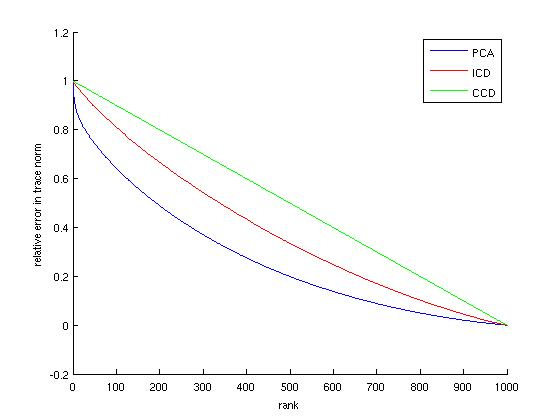
\includegraphics[width=0.5\textwidth]{trace_residual.jpg}
%    \caption{Residual error of decompositions varying by its rank.}
%    \label{fig:residue}
%\end{figure}

